\documentclass{article}
\usepackage{ShumanNotes}
\usepackage{titling}

\setlength{\droptitle}{-10em}
\title{ CS261 Homework 0: Introduce Yourself}
\author{Rattanai Sawaspanich}
\date{April 3rd, 2013}
\setlength{\parindent}{35pt}
\pdfpagewidth 8.5in
\pdfpageheight 11in

\begin{document} 
\maketitle

\section{Introduction}
\centerimage{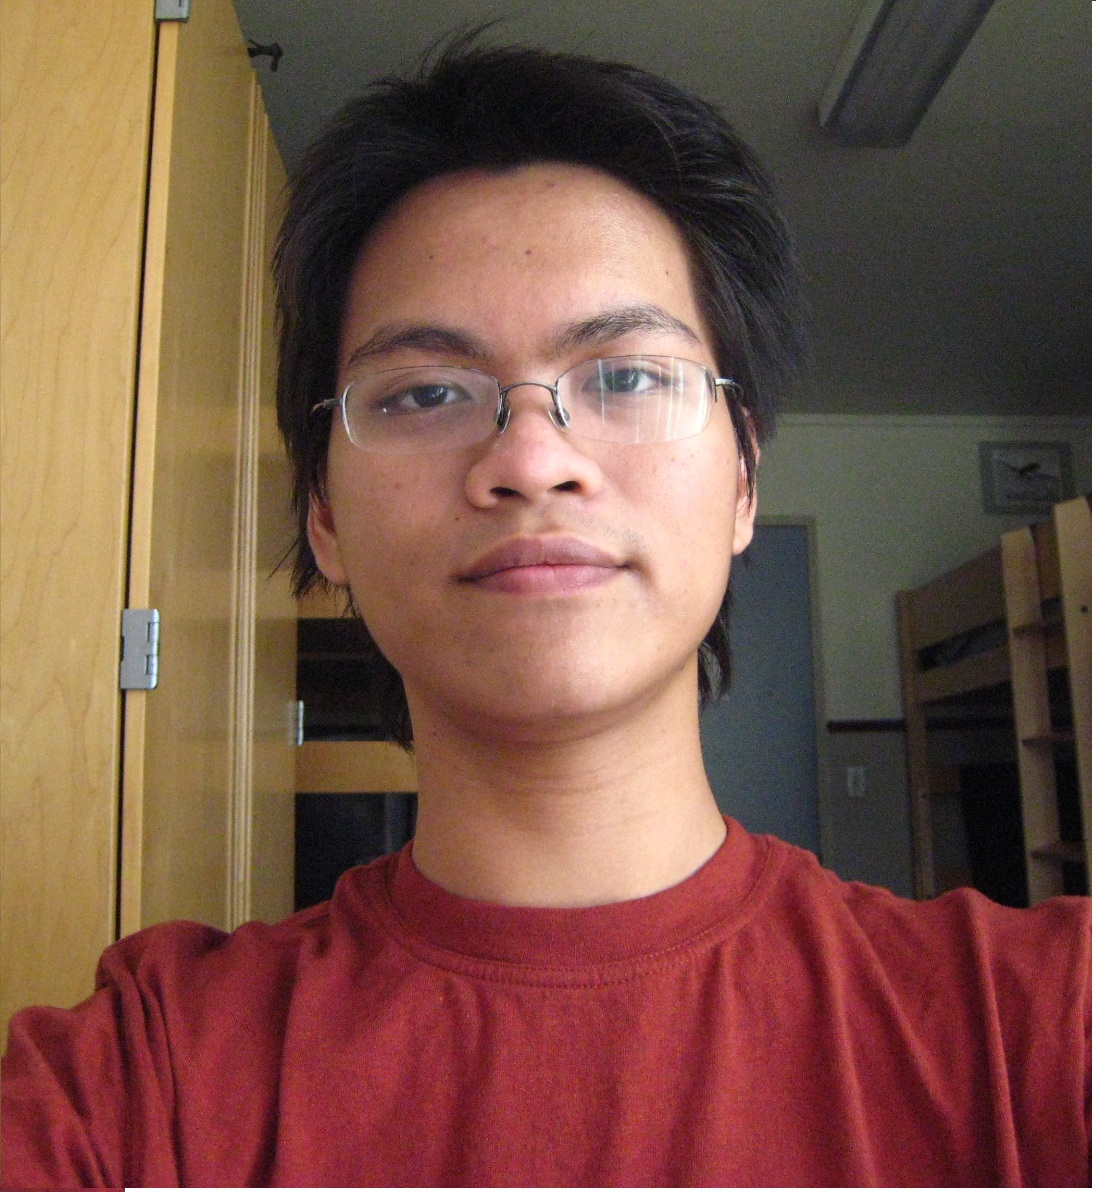
\includegraphics[width = 2in]{./IMG_0897.jpg} }{Rattanai Sawaspanich}{me}
 \indent  Hello World.  My name is Rattanai Sawaspanich but usually go by "Bear\footnote{I picked my name as "Bear" because my \emph{nickname} in Thai is 
\includegraphics[width=0.115in]{./Bear_T.jpg} which means "Bear" so I translated it to English.}".  I am a freshman at OSU studying Electrical and Computer Engineering. I am Thai. I have a total of three siblings: me, the oldest son, my younger sister, 16, and my younger brother, 10.  Our family owns an auto-mobile garage; my dad is a head-mechanic as well as the owner of the business and my mom helps my dad manage the business' finances. 
\newline \indent  The motivation that drew me to the U.S. was that I would like to expand my perspective of the world. I applied and was accepted to be a participant in the AFS exchange program while I was a junior in high school.Through the AFS program, I spent that year studying in the US. I have learned so many things from this different perspective, and I like it here, so I decided to continue my education in the US.  I applied to colleges and got into OSU as an Electical and Computer Engineering major.  My career goal is to work in the field of Quantum Computing. I want to be working in this field because its concepts are very bizzare, intriguing, and contain the potential to be very useful to mankind.  I can see myself as a researcher in Quantum Computing ten years from now.


\section{Programming Experience}
\begin{itemize}
\item Visual Basic - I first started programming in Visual Basic 6 about four years ago but I have not looked into it much in the last two years because I was busy learning English and adjusting to the culture difference. I would say my programming in VB is capable. 
\item HTML - I spent a summer creating a webpage for my friend with HTML so I think  my HTML skill is in between novice and capable.
\item C++/C - I recently began learning C/C++ in CS161, fall term, taught by Prof. Jennifer.  Then, I learned more in CS162 last term. Compared with the potential of what C/C++ can do, I consider myself a novice.


\end{itemize}




\cfoot{CS 261 Homework 0}

\end{document}
